\section{Đặc tả chi tiết các lược đồ hệ thống}

Khắc phục hạn chế thiếu trực quan hóa kiến trúc thường gặp ở các báo cáo giai đoạn đầu, chương này trình bày đầy đủ hệ thống lược đồ UML và luồng xử lý của \textit{Convergence Chess} ở các mức độ từ nghiệp vụ người dùng (Use-case) đến thiết kế lớp (Class), tương tác tuần tự (Sequence), máy trạng thái (State) và quy trình dữ liệu (Pipeline). Toàn bộ lược đồ nguồn dạng \texttt{.drawio} và \texttt{.puml} được lưu đồng bộ tại thư mục \texttt{Diagrams/} của kho mã nguồn báo cáo để thuận tiện bảo trì sang Giai đoạn 2 (DATN).

\subsection{Lược đồ Use-case tổng thể và đặc tả kịch bản chính}
Hình \ref{fig:usecase_overview} mô tả tổng thể các tác nhân (Người chơi chính, Đối thủ Online/Offline, Khán giả và Bot AI) cùng 12 ca sử dụng (Use-case) trải dài từ khâu chuẩn bị đội hình, quản lý phòng chơi trực tuyến đến vòng lặp thi đấu $6 \times 6$.

\begin{figure}[H]
    \centering
    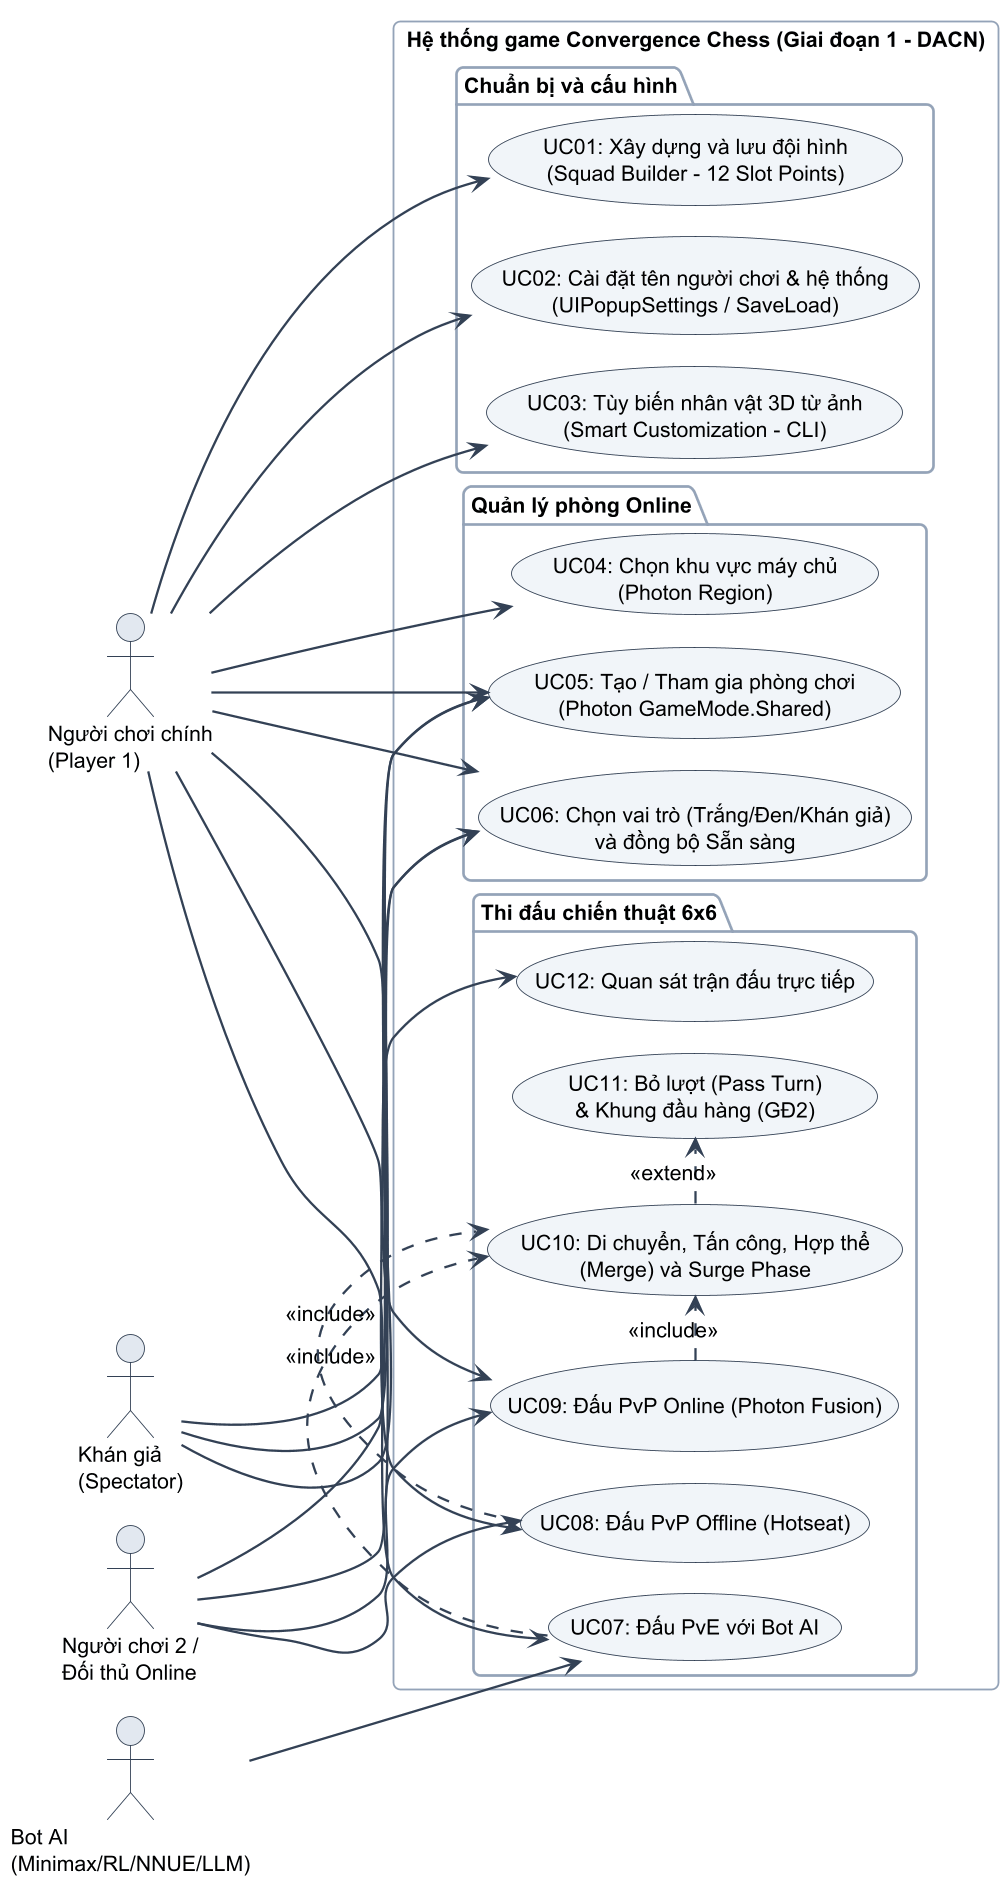
\includegraphics[width=0.72\textwidth,height=0.72\textheight,keepaspectratio]{Diagrams/images/01_usecase_overview.png}
    \caption{Lược đồ Use-case tổng thể hệ thống Convergence Chess}
    \label{fig:usecase_overview}
\end{figure}

{\small
\begin{longtable}{L{2.5cm} L{2.4cm} L{5.3cm} L{4.7cm}}
    \caption{Đặc tả kịch bản cho các Use-case trọng tâm của hệ thống}
    \label{tab:usecase_specs} \\
    \toprule
    \textbf{Use-case} & \textbf{Tác nhân và tiền điều kiện} & \textbf{Luồng sự kiện chính} & \textbf{Luồng ngoại lệ và ràng buộc} \\
    \midrule
    \endfirsthead
    \toprule
    \textbf{Use-case} & \textbf{Tác nhân và tiền điều kiện} & \textbf{Luồng sự kiện chính} & \textbf{Luồng ngoại lệ và ràng buộc} \\
    \midrule
    \endhead
    \bottomrule
    \endfoot
        UC01: Xây dựng và lưu đội hình (Squad Builder) & Người chơi chính; đang ở màn hình Main Menu. & (1) Mở \texttt{UIPopupSquadBuilder}; (2) Kéo thả quân cờ vào 12 ô sân nhà (trừ ô Vua cố định tại chỉ số 3); (3) Hệ thống tính tổng Slot Points thời gian thực theo \texttt{GameplayConfig.MaxSlotsInSquad} (hiện hành $12$ Slot Points) qua \texttt{SquadValidator}; (4) Nhấn Lưu để ghi ra \texttt{SquadSLO} qua \texttt{SaveLoadManager}. & Nếu tổng Slot Points vượt quá hạn mức cấu hình ($12$), chọn quân bị khóa (\texttt{Queen}) hoặc ô đã có quân/Vua, thao tác đặt quân bị chặn và hiển thị thông báo. \\
        \midrule
        UC05--UC06: Tạo/Vào phòng Online, phân vai và Sẵn sàng & Người chơi chính, Đối thủ Online, Khán giả; có kết nối Internet. & (1) Chọn Photon Region và nhập Room ID tại \texttt{UIPopupLobby}; (2) Host mở phòng ở chế độ \texttt{GameMode.Shared} và chiếm vị trí Trắng; (3) Client tham gia, gửi tên người chơi (\texttt{MSG\_MAP\_PLAYER\_NAME}) và yêu cầu đồng bộ slot (\texttt{MSG\_REQUEST\_SLOT\_SYNC}); (4) Chọn vị trí Trắng/Đen/Khán giả, chọn Squad và bật Ready; (5) Khi cả Trắng và Đen sẵn sàng, Host sinh \texttt{MatchSeed} + vật cản và phát \texttt{MSG\_MATCH\_INIT} để đồng loạt tải \texttt{PvPOnlScene}. & Nếu phòng đầy 2 người chơi chính, người vào sau tự động xếp vào danh sách Khán giả (\texttt{Spectator}). Nếu mất kết nối Photon Cloud, hiển thị trạng thái lỗi trên \texttt{OnConnectionStatusChanged}. \\
        \midrule
        UC10--UC11: Thực hiện nước đi, Hợp thể và Surge Phase & Người chơi đang tới lượt hoặc Bot AI; trận đấu đang ở trạng thái \texttt{WaitingInput}. & (1) Chọn quân đồng minh, hệ thống highlight ô hợp lệ; (2) Chọn ô đích để Di chuyển, Tấn công hoặc Hợp thể; (3) \texttt{MoveValidator.ValidateAction} xác thực, \texttt{GameEventHandler.ExecuteCommand} cập nhật \texttt{GameState} và phát \texttt{GameEventBatch}; (4) Nếu vừa Hợp thể và còn đủ AP, mở \texttt{Surge Sub-phase} cho phép đánh bồi hoặc kết thúc lượt giữ AP; (5) Chuyển lượt. & Không đủ AP, chọn ô vật cản với quân trượt, hợp thể 2 quân cùng loại hoặc hợp thể quân đã có \texttt{HasMerged = true} đều bị từ chối. Bỏ lượt bị chặn khi \texttt{PassChargesLeft == 0}; nếu không còn nước đi hợp lệ nào, phe tới lượt bị xử thua. \\
        \midrule
        UC03: Tùy biến nhân vật 3D từ ảnh chân dung (SC) & Người chơi chính; môi trường Python cục bộ chứa \texttt{infer\_onnx.py} và trọng số ONNX/HRN sẵn sàng. & (1) Mở giao diện \texttt{SCCanvasUI}, chọn giới tính (Nam/Nữ), chế độ texture (\texttt{TexNet}/\texttt{HRN}) và ảnh chân dung 2D; (2) \texttt{SCCharacterCreator} khởi chạy tiến trình con \texttt{infer\_onnx.py} qua \texttt{ProcessStartInfo}; (3) Đọc \texttt{sc\_result.json}, ảnh da khử bóng và Normal Map trên ổ đĩa; (4) Tự động áp 25 BlendShapes, màu mắt, màu tóc và cho phép tinh chỉnh thanh trượt hoặc đổi 7 kiểu tóc 3D. & Nếu ảnh không phát hiện khuôn mặt qua MediaPipe hoặc tiến trình Python trả mã lỗi, Unity giữ nguyên nhân vật cơ sở và hiển thị thông báo lỗi mà không treo ứng dụng. \\
\end{longtable}
}

\subsection{Lược đồ kiến trúc tổng thể (Hexagonal Architecture -- Ports \& Adapters)}
Hình \ref{fig:arch_hexagonal} minh họa kiến trúc lục giác (Ports \& Adapters) \cite{cockburn} là xương sống của toàn bộ dự án. Toàn bộ thực thể và quy tắc thẩm định nằm trong khối \textbf{Core Domain} tách khỏi đồ họa, được điều phối vòng lặp bởi \texttt{MatchManager}. Mọi nguồn điều khiển (chuột người chơi, Photon Fusion mạng, các họ Bot AI) đều giao tiếp qua cổng \texttt{IMoveInputProvider}, còn mọi thành phần tiêu thụ kết quả (diễn hoạt 3D, xoay bàn PvP Offline, ghi nhận trận benchmark qua \texttt{BenchmarkGameEventManager}, định hình thưởng \texttt{AgentRewardHandler} hoặc \texttt{NullGameEventListener} cho huấn luyện Headless) đều đi qua cổng \texttt{IGameEventListener} dưới sự điều phối cục bộ của \texttt{ArenaServiceLocator}.

\begin{figure}[H]
    \centering
    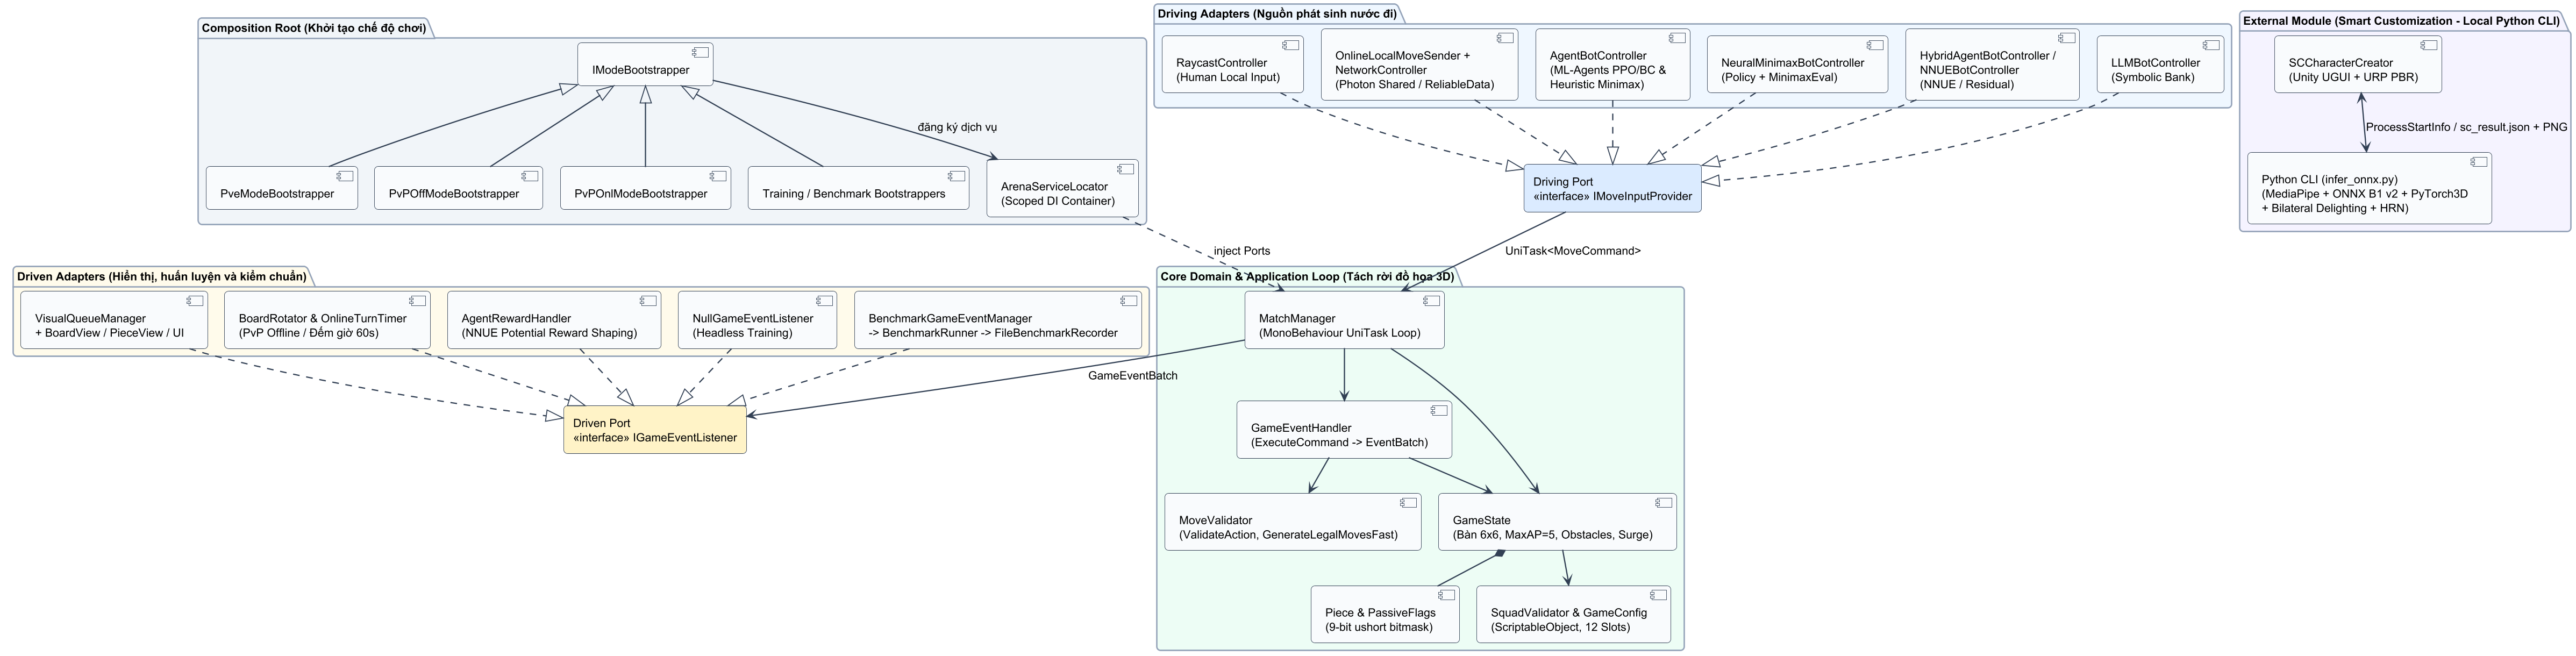
\includegraphics[width=\textwidth]{Diagrams/images/02_architecture_hexagonal.png}
    \caption{Sơ đồ kiến trúc tổng thể theo mô hình Ports \& Adapters và ArenaServiceLocator}
    \label{fig:arch_hexagonal}
\end{figure}

\subsection{Lược đồ lớp (Class diagrams) theo từng phân hệ}
Để bảo đảm khả năng đọc rõ ràng trên khổ giấy A4, lược đồ lớp toàn hệ thống được phân tách thành ba phân hệ chính khớp trực tiếp với cấu trúc thư mục mã nguồn trong \texttt{Assets/Scripts/}.

\subsubsection{Lược đồ lớp phân hệ Core Logic và các bộ điều khiển AI}
Hình \ref{fig:class_core_ai} thể hiện quan hệ giữa \texttt{MatchManager}, \texttt{GameEventHandler}, \texttt{GameState}, \texttt{Piece}, \texttt{MoveValidator} và các lớp thực thi \texttt{IMoveInputProvider} phục vụ AI (\texttt{AgentBotController}, \texttt{NeuralMinimaxBotController}, \texttt{HybridAgentBotController}, \texttt{NNUEBotController}, \texttt{LLMBotController}) kết nối tới \texttt{ObservationEncoderV2}, \texttt{MinimaxSearch}, \texttt{NNUEFastEvaluator}/\texttt{NNUEModelWeights} và \texttt{LLMSymbolicEvaluator}.

\begin{figure}[H]
    \centering
    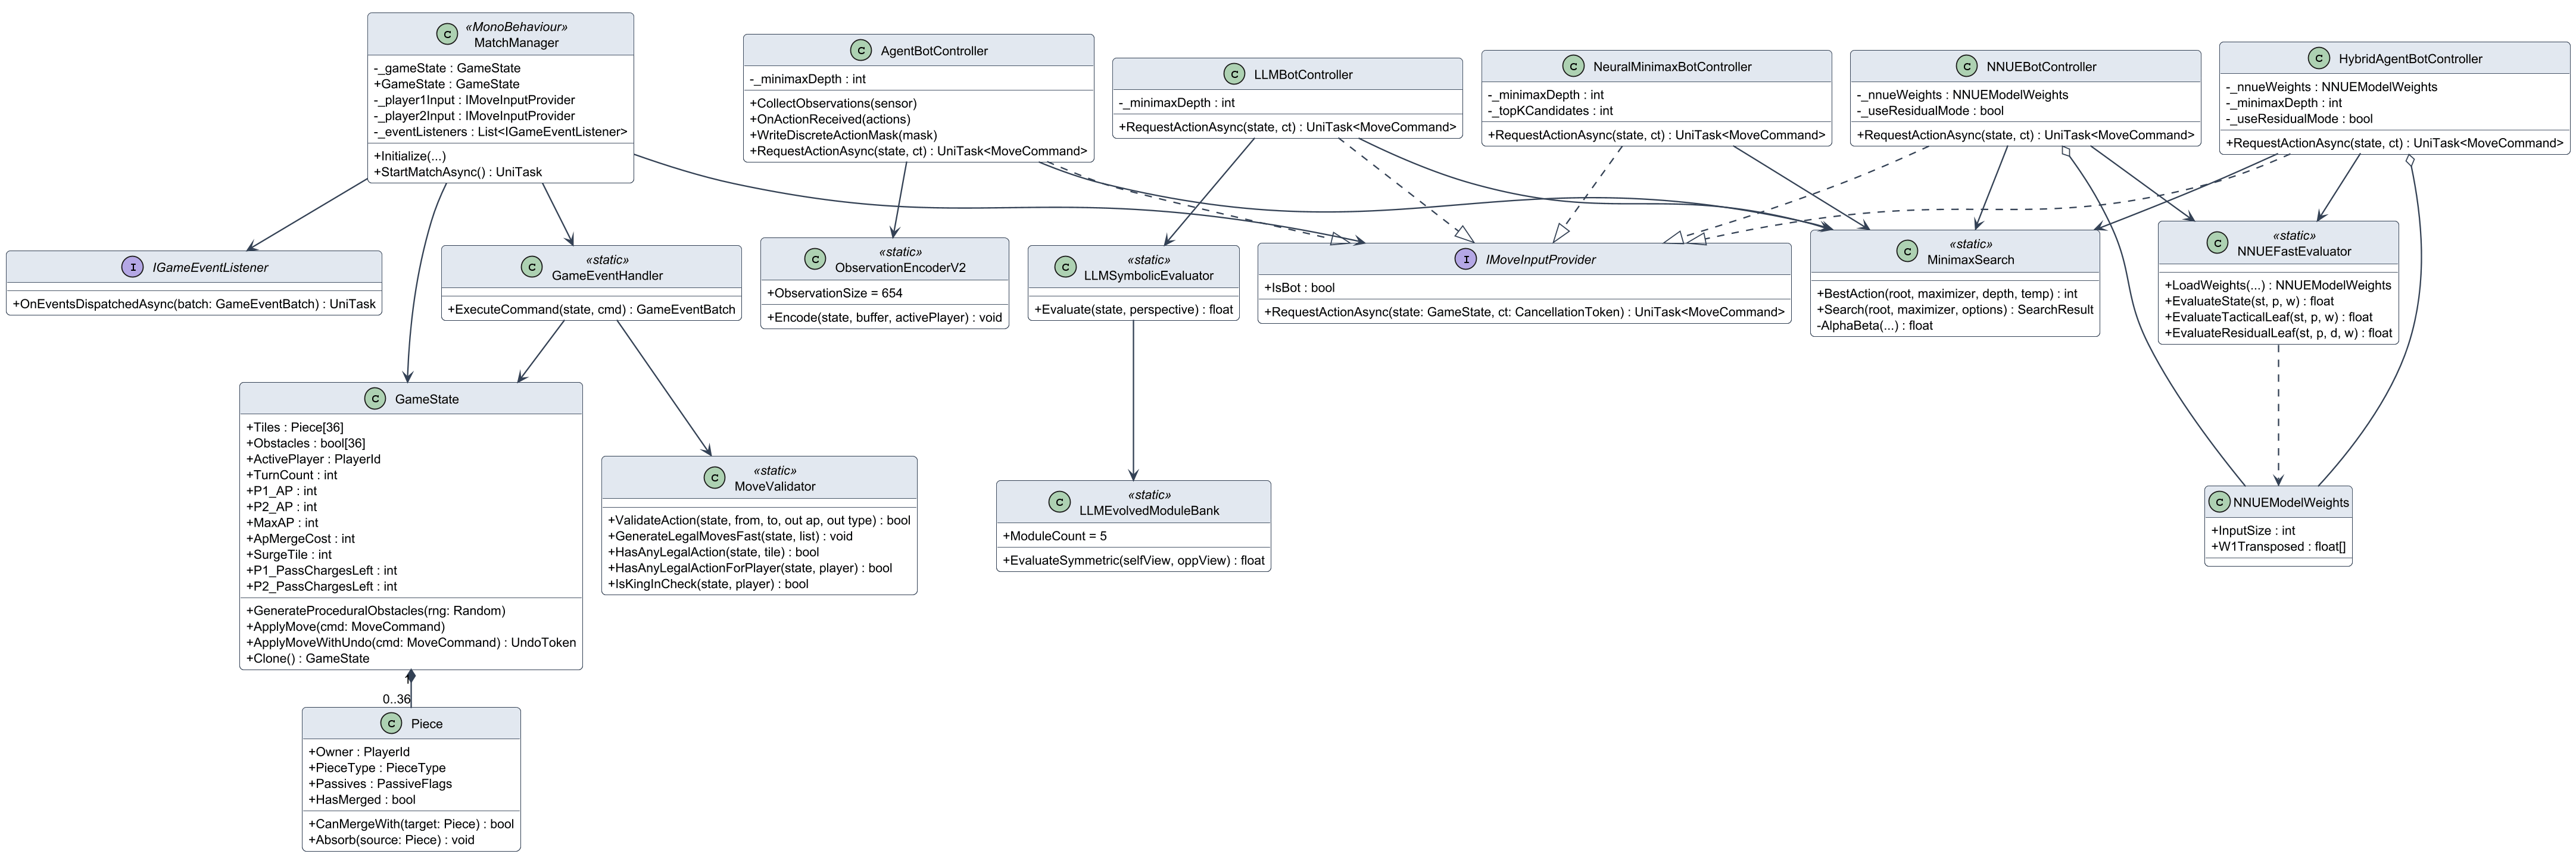
\includegraphics[width=\textwidth]{Diagrams/images/03_class_core_ai.png}
    \caption{Lược đồ lớp phân hệ Core Domain và các tác nhân AI}
    \label{fig:class_core_ai}
\end{figure}

\subsubsection{Lược đồ lớp phân hệ Multiplayer (Photon Fusion)}
Hình \ref{fig:class_network} trình bày kiến trúc mạng tách lớp: \texttt{OnlineSessionManager} điều phối phiên Photon Fusion (\texttt{GameMode.Shared}) và ủy quyền toàn bộ mã hóa/giải mã gói tin nhị phân cho \texttt{OnlineDataBroadcastNetwork}. Lớp định tuyến này sử dụng Factory Method khởi tạo đúng lớp xử lý con kế thừa \texttt{BroadcastDataHandler} dựa trên byte định danh \texttt{BroadcastDataIdentifierByte}. Ở biên giao tiếp với Core, \texttt{NetworkController} (nhận nước đi từ xa qua \texttt{UniTaskCompletionSource}) và \texttt{OnlineLocalMoveSender} (bọc \texttt{RaycastController} để phát nước đi lên mạng) cùng cài đặt \texttt{IMoveInputProvider}.

\begin{figure}[H]
    \centering
    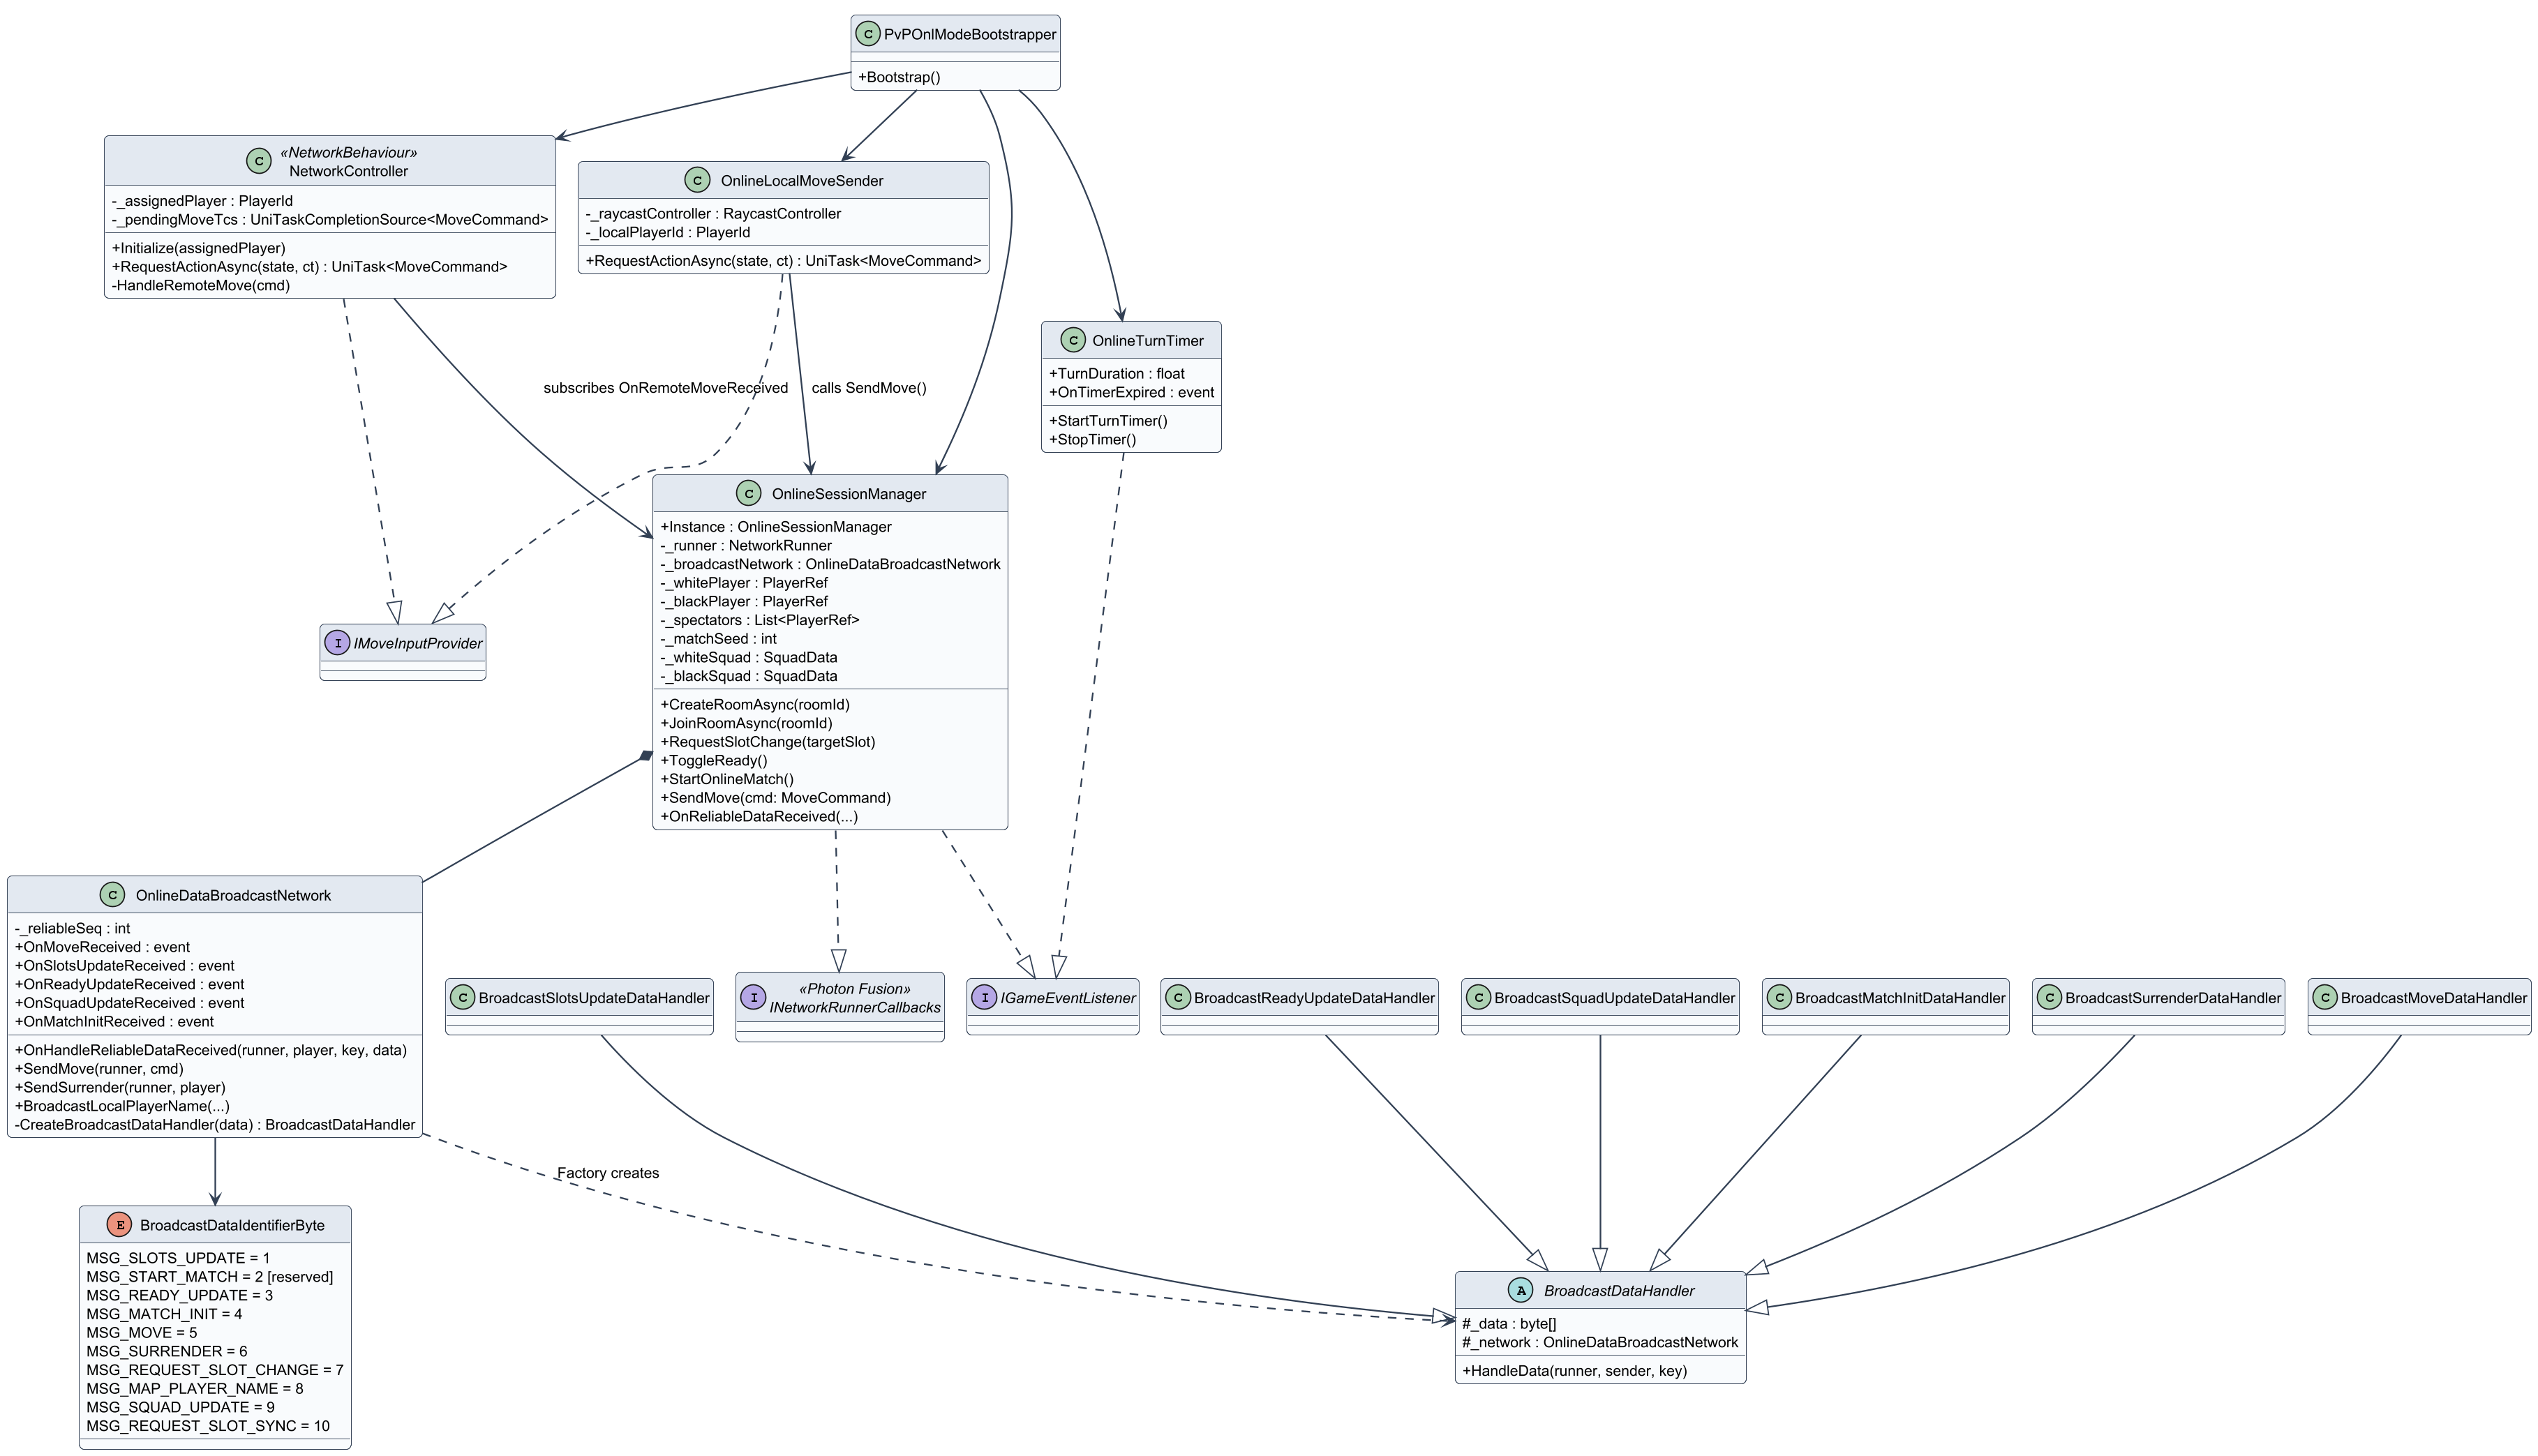
\includegraphics[width=\textwidth]{Diagrams/images/04_class_network.png}
    \caption{Lược đồ lớp phân hệ Multiplayer sử dụng Photon Fusion Reliable Data}
    \label{fig:class_network}
\end{figure}

\subsubsection{Lược đồ lớp phân hệ View Layer và giao diện người dùng (UI)}
Hình \ref{fig:class_view_ui} minh họa luồng trình diễn tách biệt hoàn toàn khỏi Core: \texttt{VisualQueueManager} lắng nghe \texttt{GameEventBatch}, sử dụng \texttt{VisualSequenceBuilder} theo phong cách chuỗi lệnh (\texttt{Then}/\texttt{PlayAsync}) để điều phối các nút diễn hoạt \texttt{IVisualNode} (\texttt{PieceMoveNode}, \texttt{PieceAttackVisualNode}...) tác động lên \texttt{BoardView}, \texttt{TileView} và \texttt{PieceView}. Sự kiện khung hình từ Animator được gom về một đầu mối duy nhất \texttt{PieceAnimationRelay}. Hệ thống giao diện sử dụng \texttt{UIManager} tra cứu prefab tập trung thông qua ScriptableObject \texttt{UIMapper} (Single Source of Truth).

\begin{figure}[H]
    \centering
    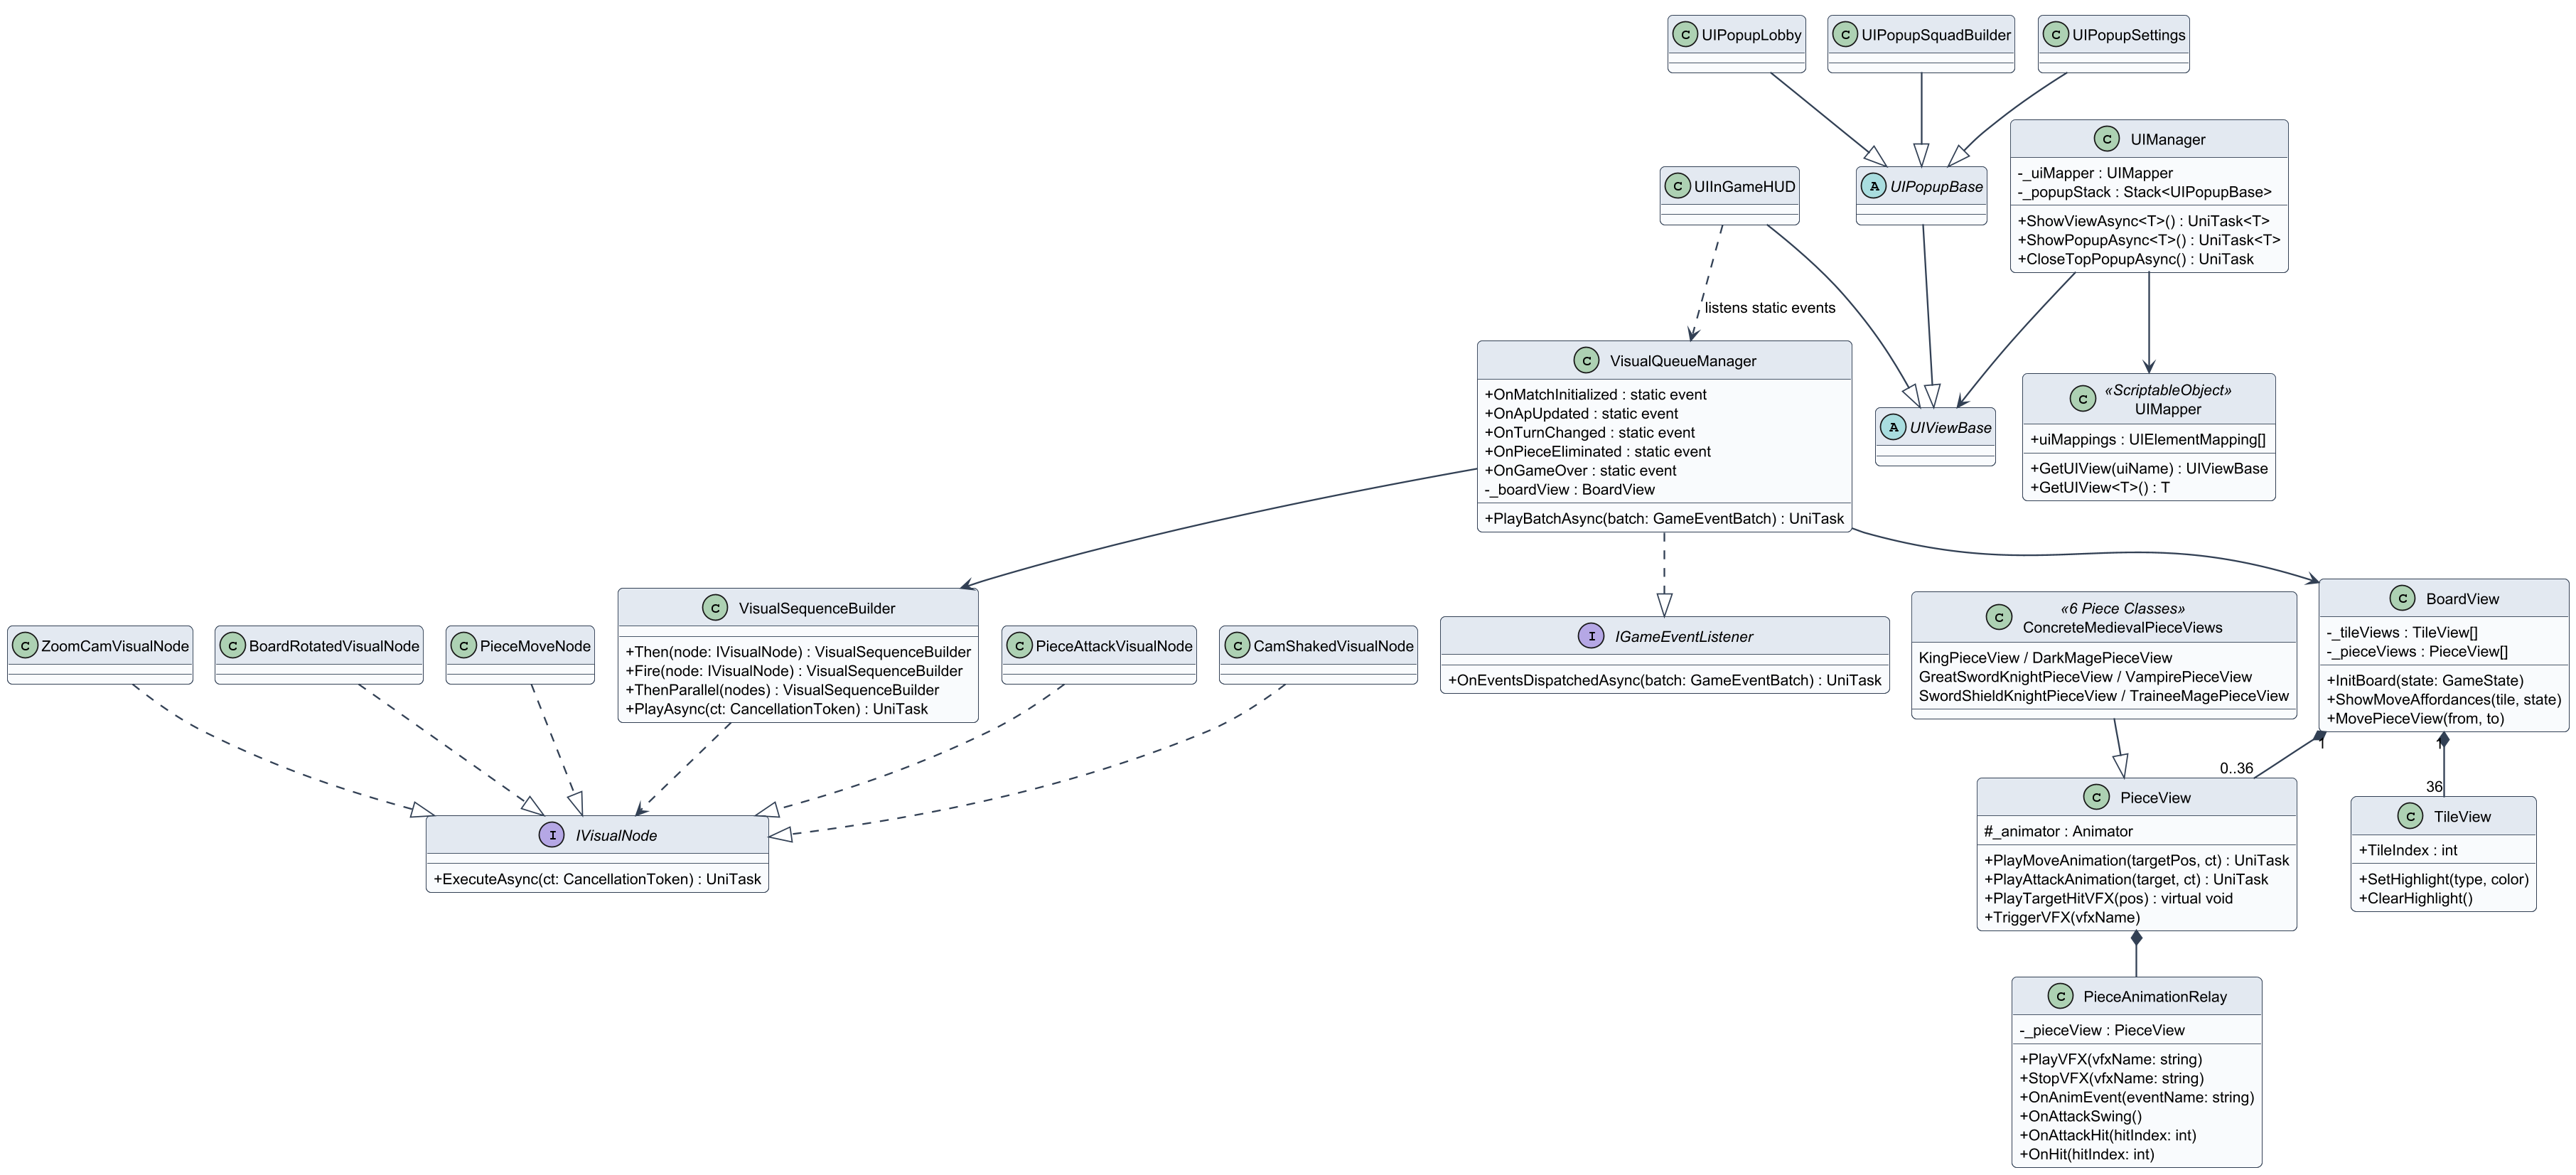
\includegraphics[width=\textwidth]{Diagrams/images/05_class_view_ui.png}
    \caption{Lược đồ lớp phân hệ View Layer, VisualQueueManager và UIManager/UIMapper}
    \label{fig:class_view_ui}
\end{figure}

\subsection{Lược đồ tuần tự (Sequence diagrams) cho luồng Multiplayer Online}
\subsubsection{Luồng khởi tạo phòng, phân vai, đồng bộ đội hình và bắt đầu trận}
Hình \ref{fig:seq_lobby} chi tiết hóa toàn bộ giao thức trao đổi gói tin tin cậy giữa máy Host (Shared Mode Master Client), Photon Fusion Cloud và máy Client từ lúc mở phòng cho tới khi hai máy đồng bộ tuyệt đối cùng một hạt giống bản đồ (\texttt{MatchSeed}), danh sách vật cản trung tuyến và đội hình hai bên.

\begin{figure}[H]
    \centering
    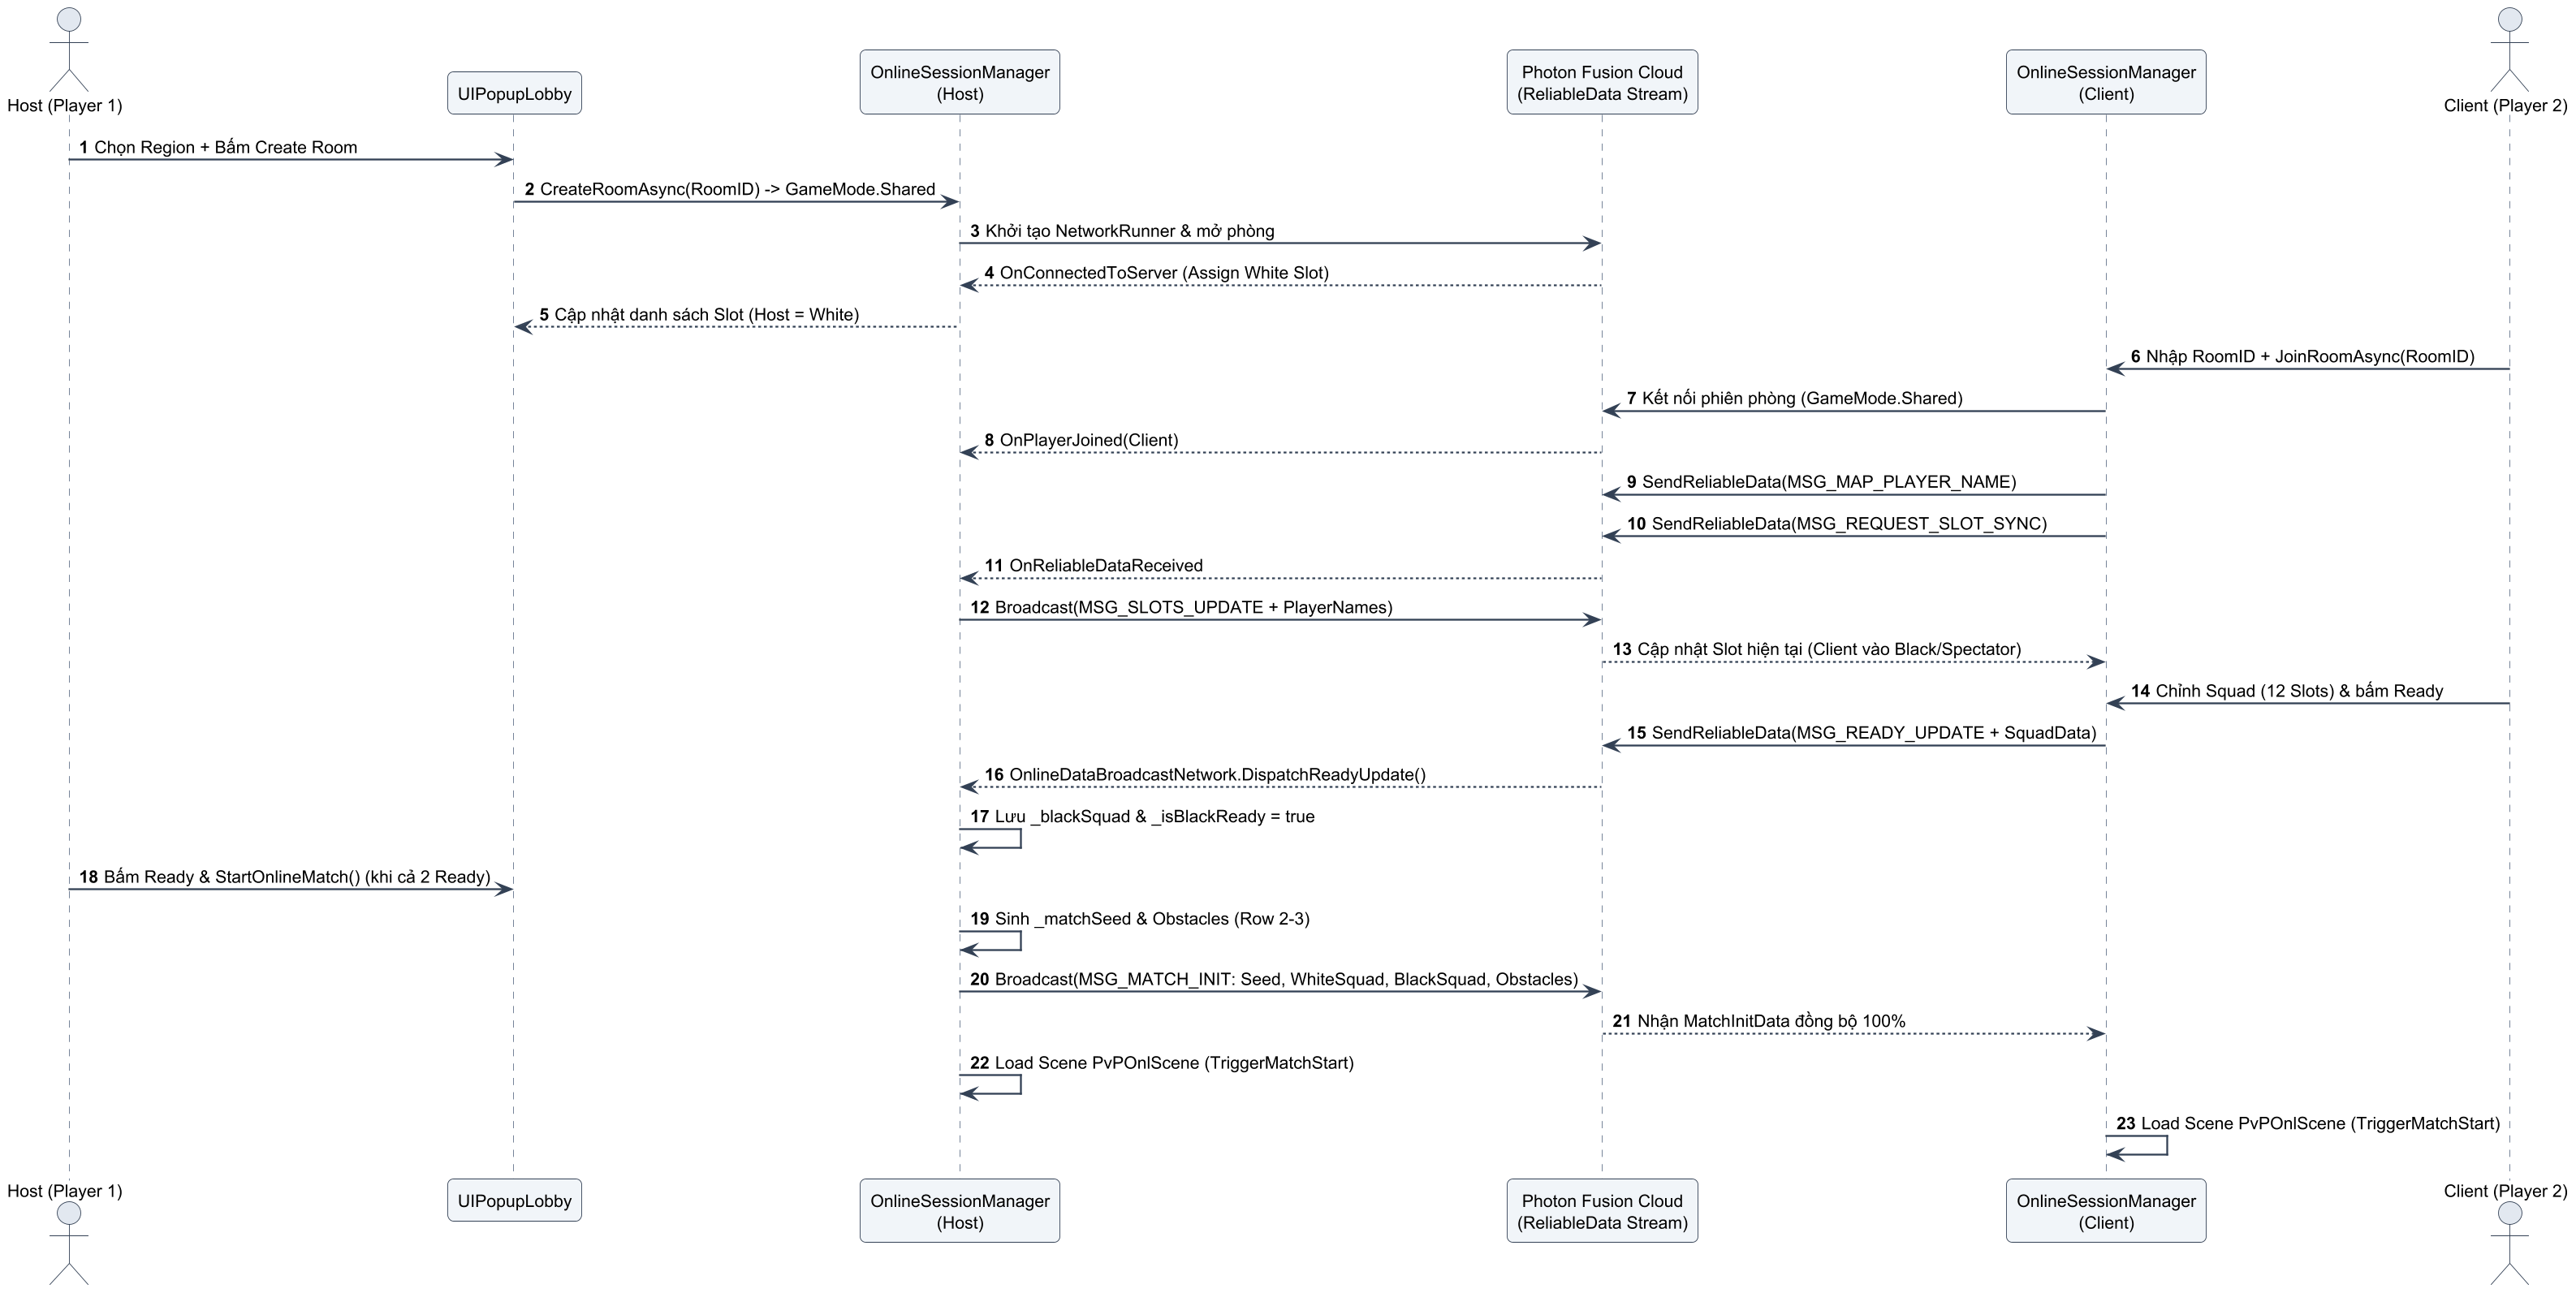
\includegraphics[width=\textwidth]{Diagrams/images/06_seq_pvp_online_lobby.png}
    \caption{Lược đồ tuần tự luồng Lobby, phân vai, đồng bộ đội hình và khởi tạo trận đấu PvP Online}
    \label{fig:seq_lobby}
\end{figure}

\subsubsection{Luồng truyền và thực thi một nước đi hợp lệ trong PvP Online}
Hình \ref{fig:seq_move} mô tả cơ chế đồng bộ nước đi khép kín chỉ với \textbf{4 bytes payload nhị phân} (\texttt{[MSG\_MOVE, FromTile, ToTile, PlayerId]}). Nhờ lõi \texttt{GameState} và \texttt{GameEventHandler} mang tính tất định (Deterministic), khi nước đi hợp lệ được xác nhận cục bộ và phát tới đối thủ qua Photon Reliable Data, cả hai máy đều tự cập nhật trạng thái ván đấu và diễn hoạt độc lập qua \texttt{VisualQueueManager} mà không cần truyền vị trí 3D liên tục từng khung hình.

\begin{figure}[H]
    \centering
    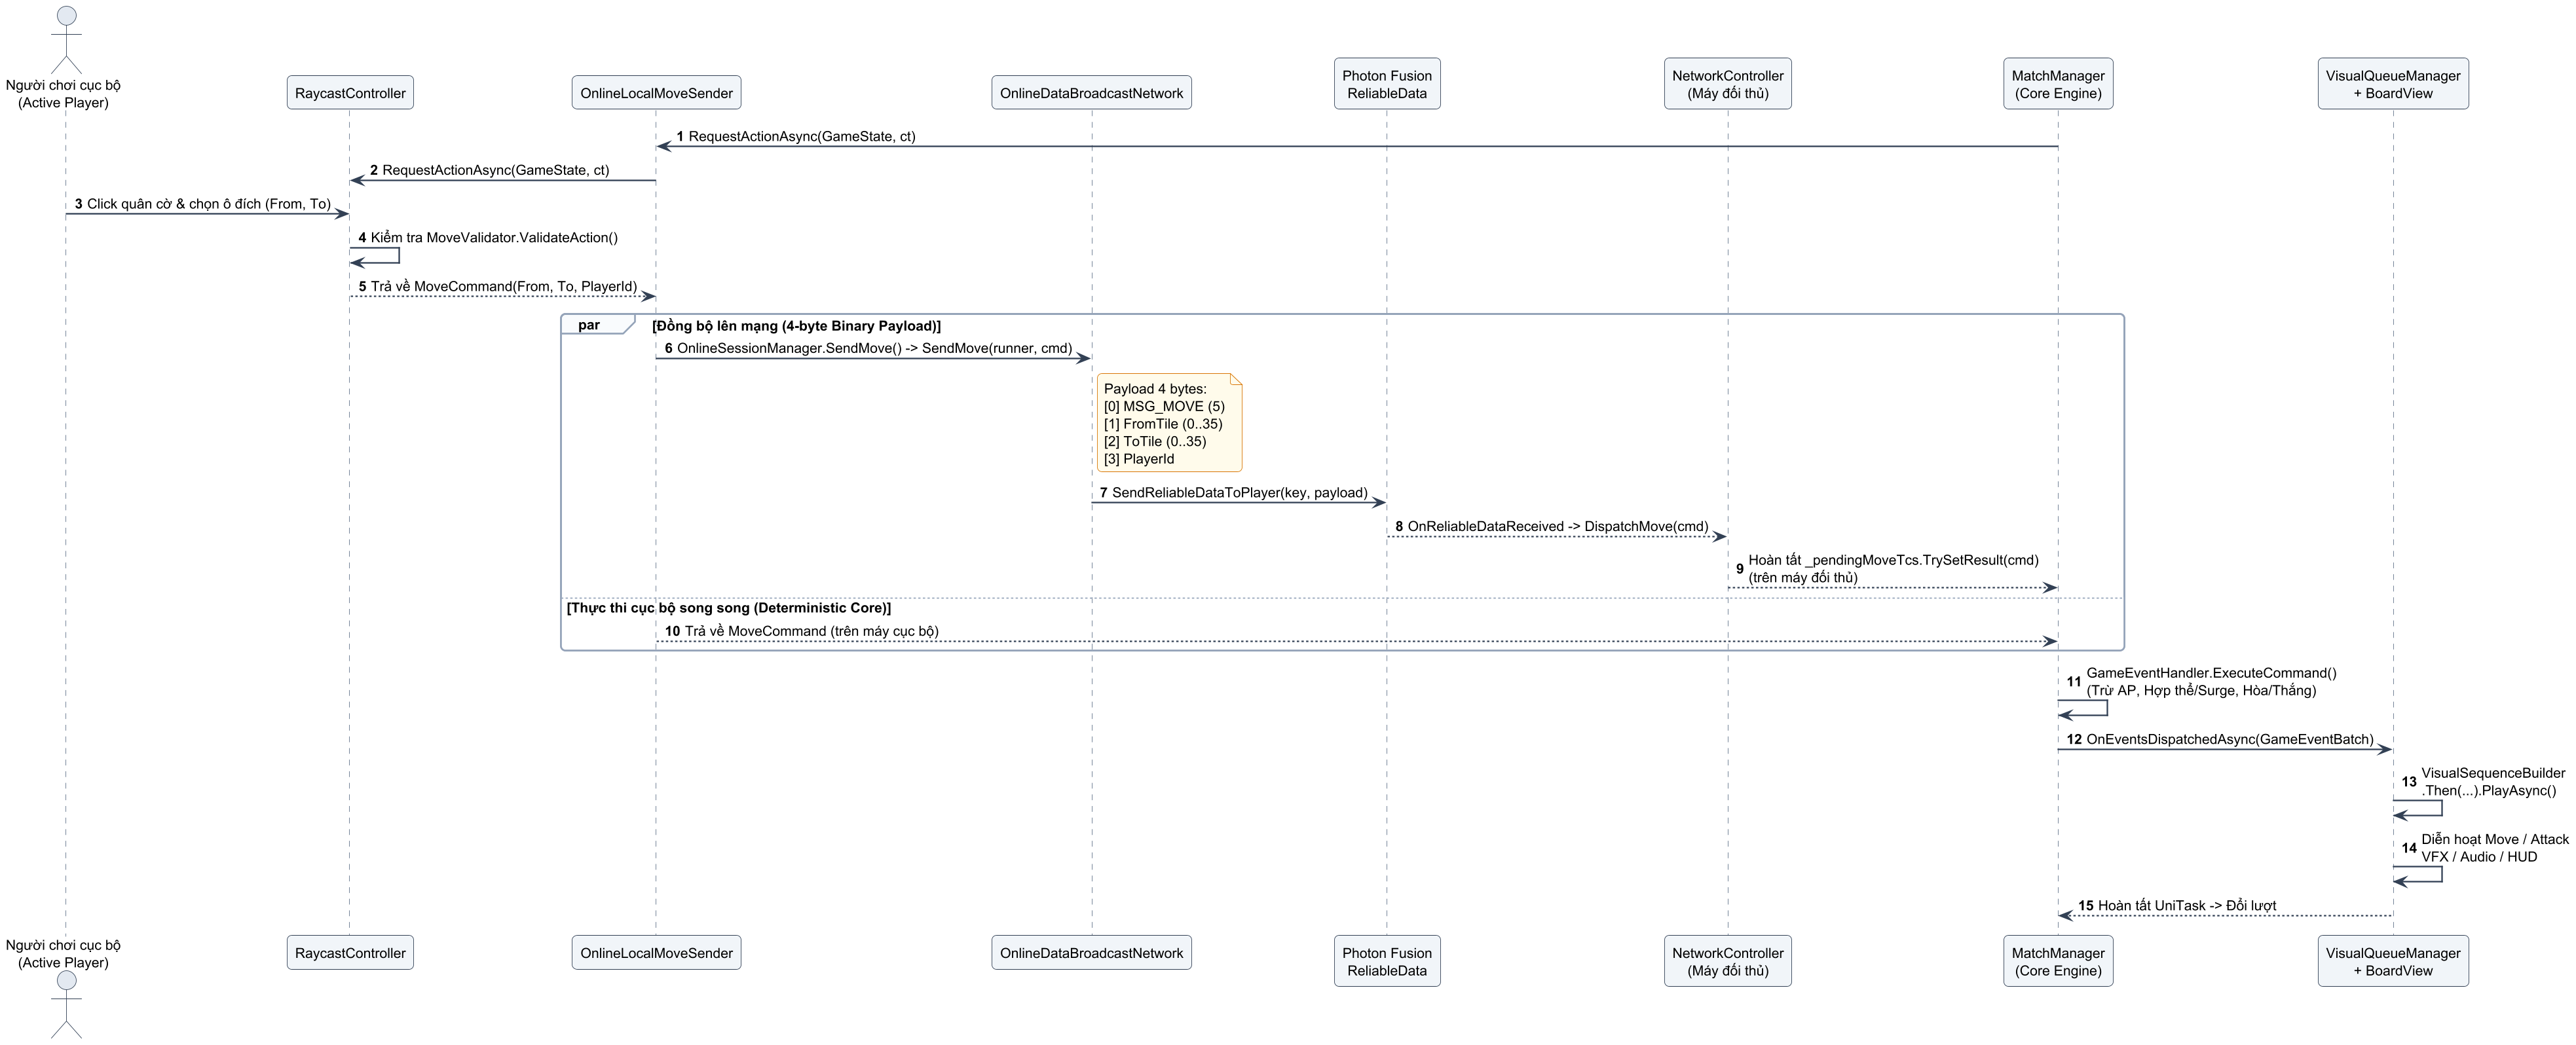
\includegraphics[width=\textwidth]{Diagrams/images/07_seq_pvp_online_move.png}
    \caption{Lược đồ tuần tự luồng gửi, nhận và diễn hoạt một nước đi trong chế độ PvP Online}
    \label{fig:seq_move}
\end{figure}

\subsection{Lược đồ trạng thái (State diagrams) của ván đấu và quân cờ 3D}
Hình \ref{fig:state_machine} tổng hợp hai máy trạng thái quan trọng nhất: (i) vòng đời một trận đấu trong \texttt{MatchManager}/\texttt{GameEventHandler}/\texttt{GameState} thể hiện rõ nhánh chuyển sang \texttt{SurgeSubPhase} sau khi hợp thể cùng đầy đủ các điều kiện kết thúc trận; và (ii) máy trạng thái 5 pha của \texttt{PieceView} (\texttt{IdleStateBase}, \texttt{MoveStateBase}, \texttt{AttackStateBase}, \texttt{GetHitStateBase}, \texttt{DeathStateBase} cùng các lớp con theo từng quân cờ).

\begin{figure}[H]
    \centering
    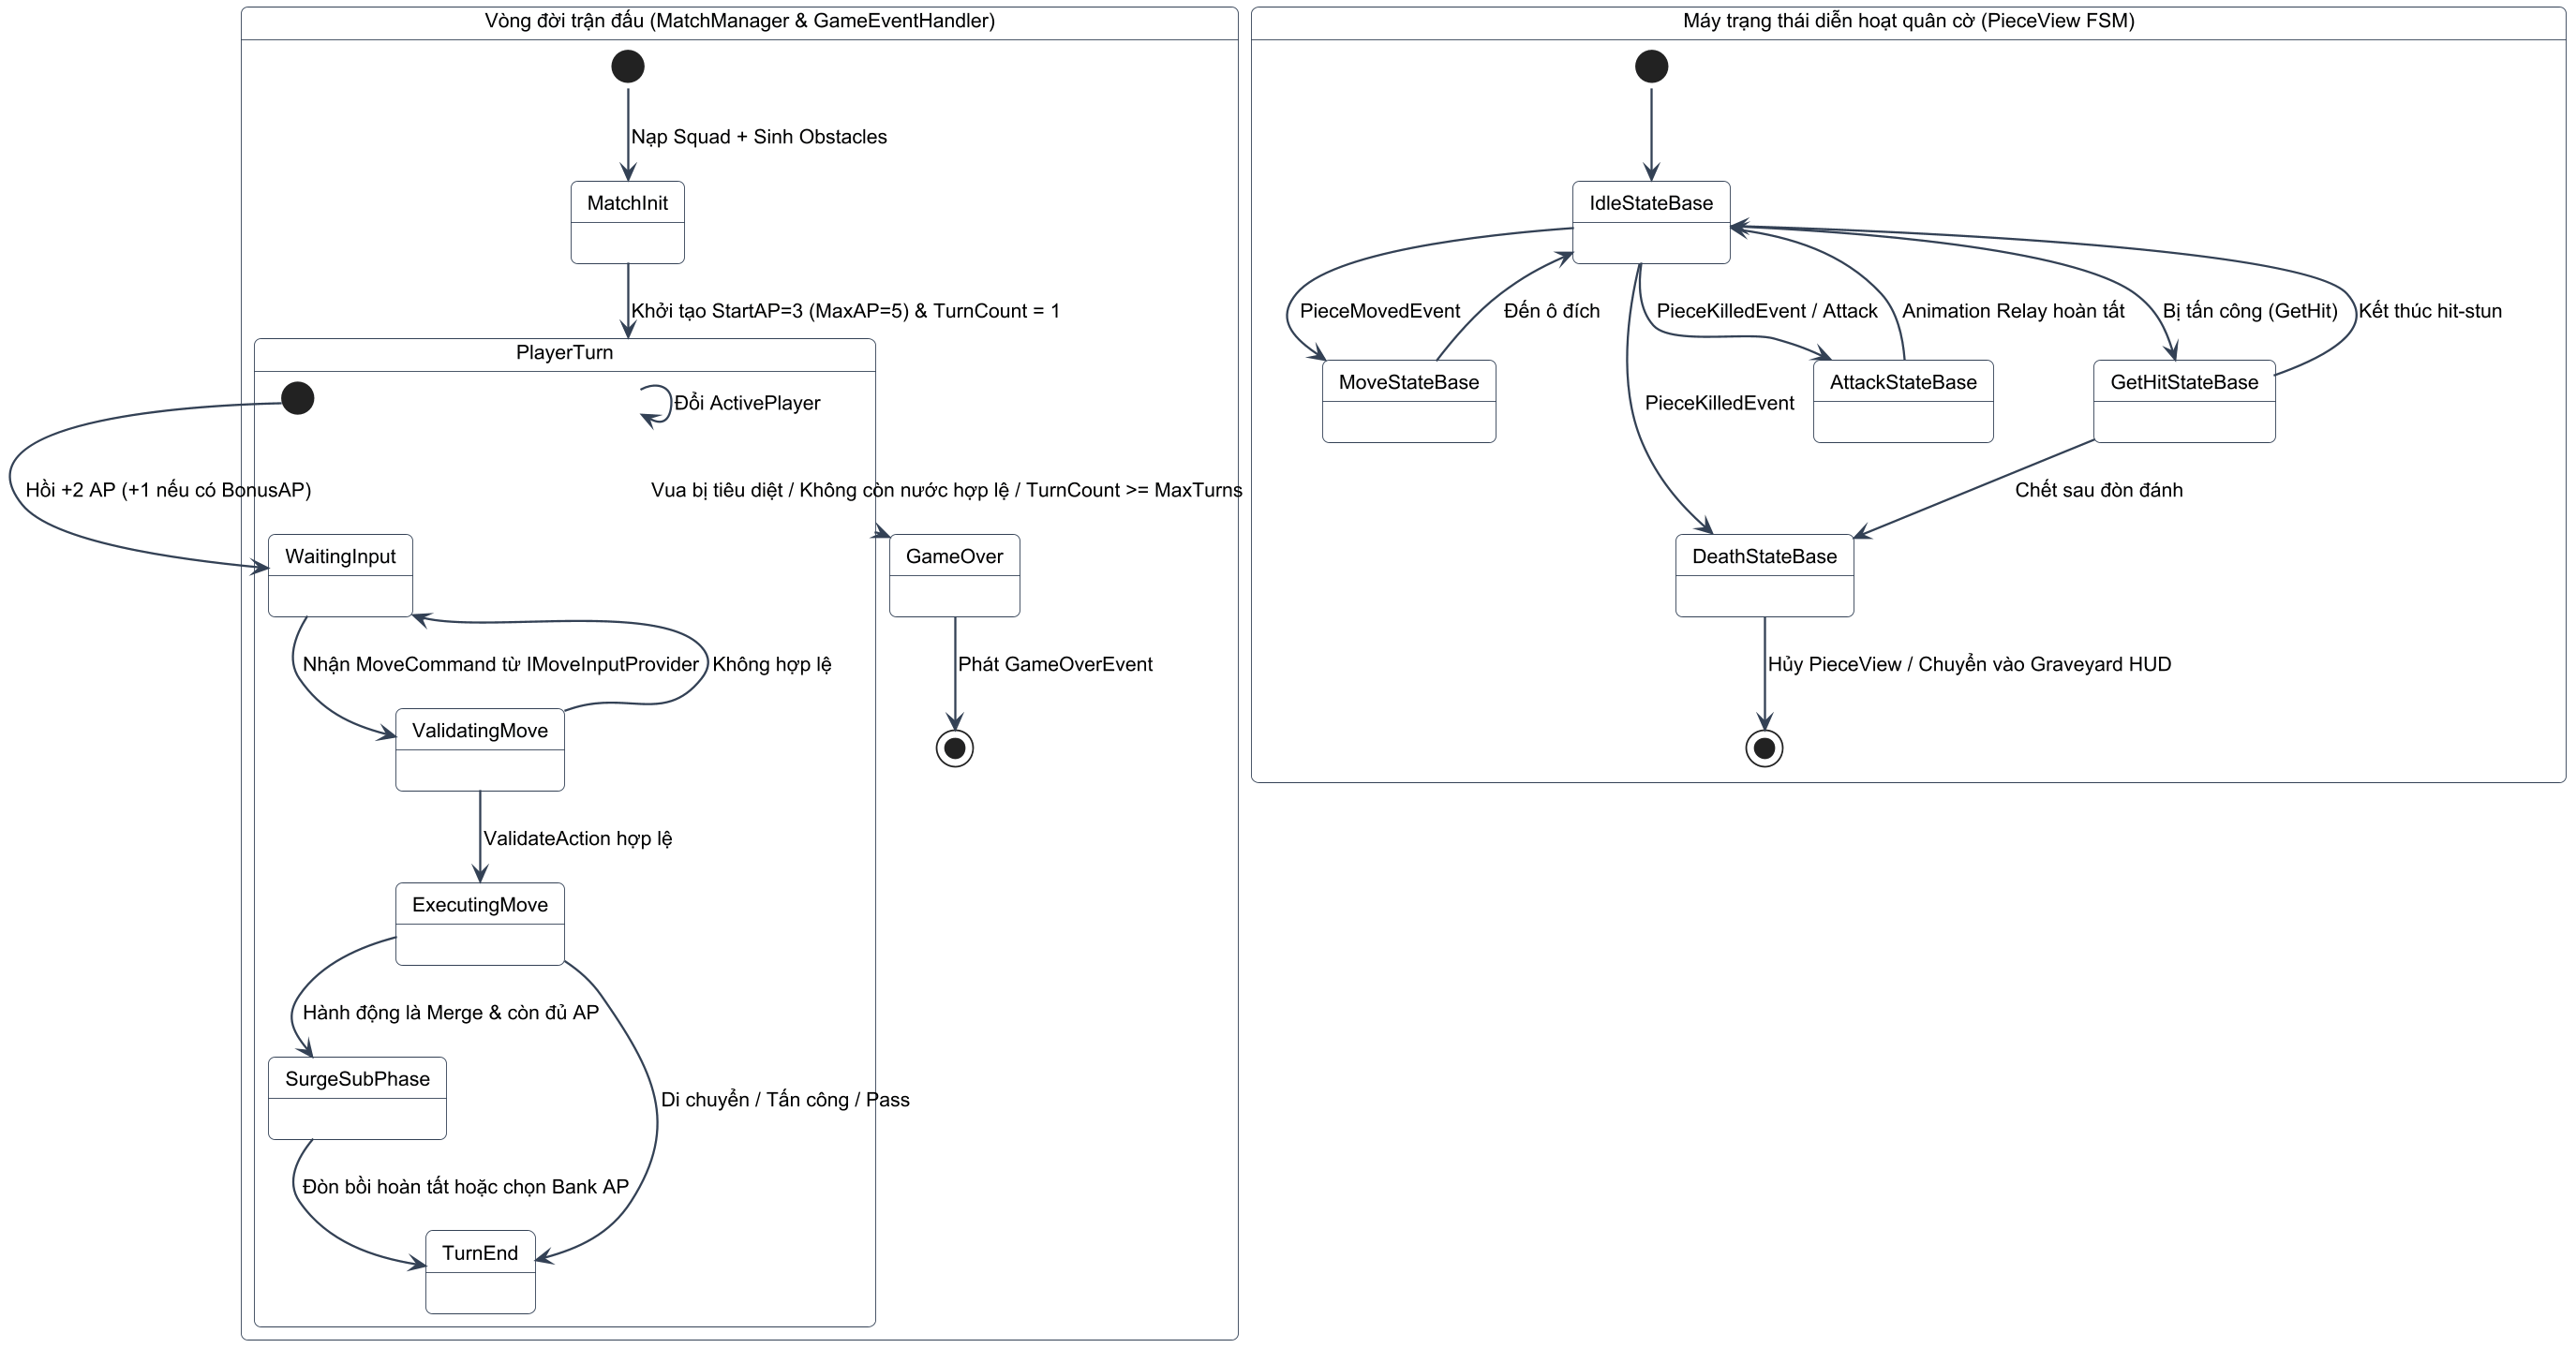
\includegraphics[width=0.96\textwidth]{Diagrams/images/08_state_piece_and_match.png}
    \caption{Lược đồ trạng thái vòng đời trận đấu (MatchManager) và diễn hoạt quân cờ (PieceView FSM)}
    \label{fig:state_machine}
\end{figure}

\subsection{Sơ đồ quy trình huấn luyện AI đa thế hệ và Smart Customization}
Hình \ref{fig:pipeline_ai} khái quát hóa hệ sinh thái 5 tầng huấn luyện và kiểm chuẩn AI trong dự án, thể hiện vòng lặp đồng huấn luyện (Iterative Co-training) giữa ML-Agents PPO và mạng giá trị NNUE/Residual NNUE cùng nhánh tiến hóa luật biểu tượng bằng LLM.

\begin{figure}[H]
    \centering
    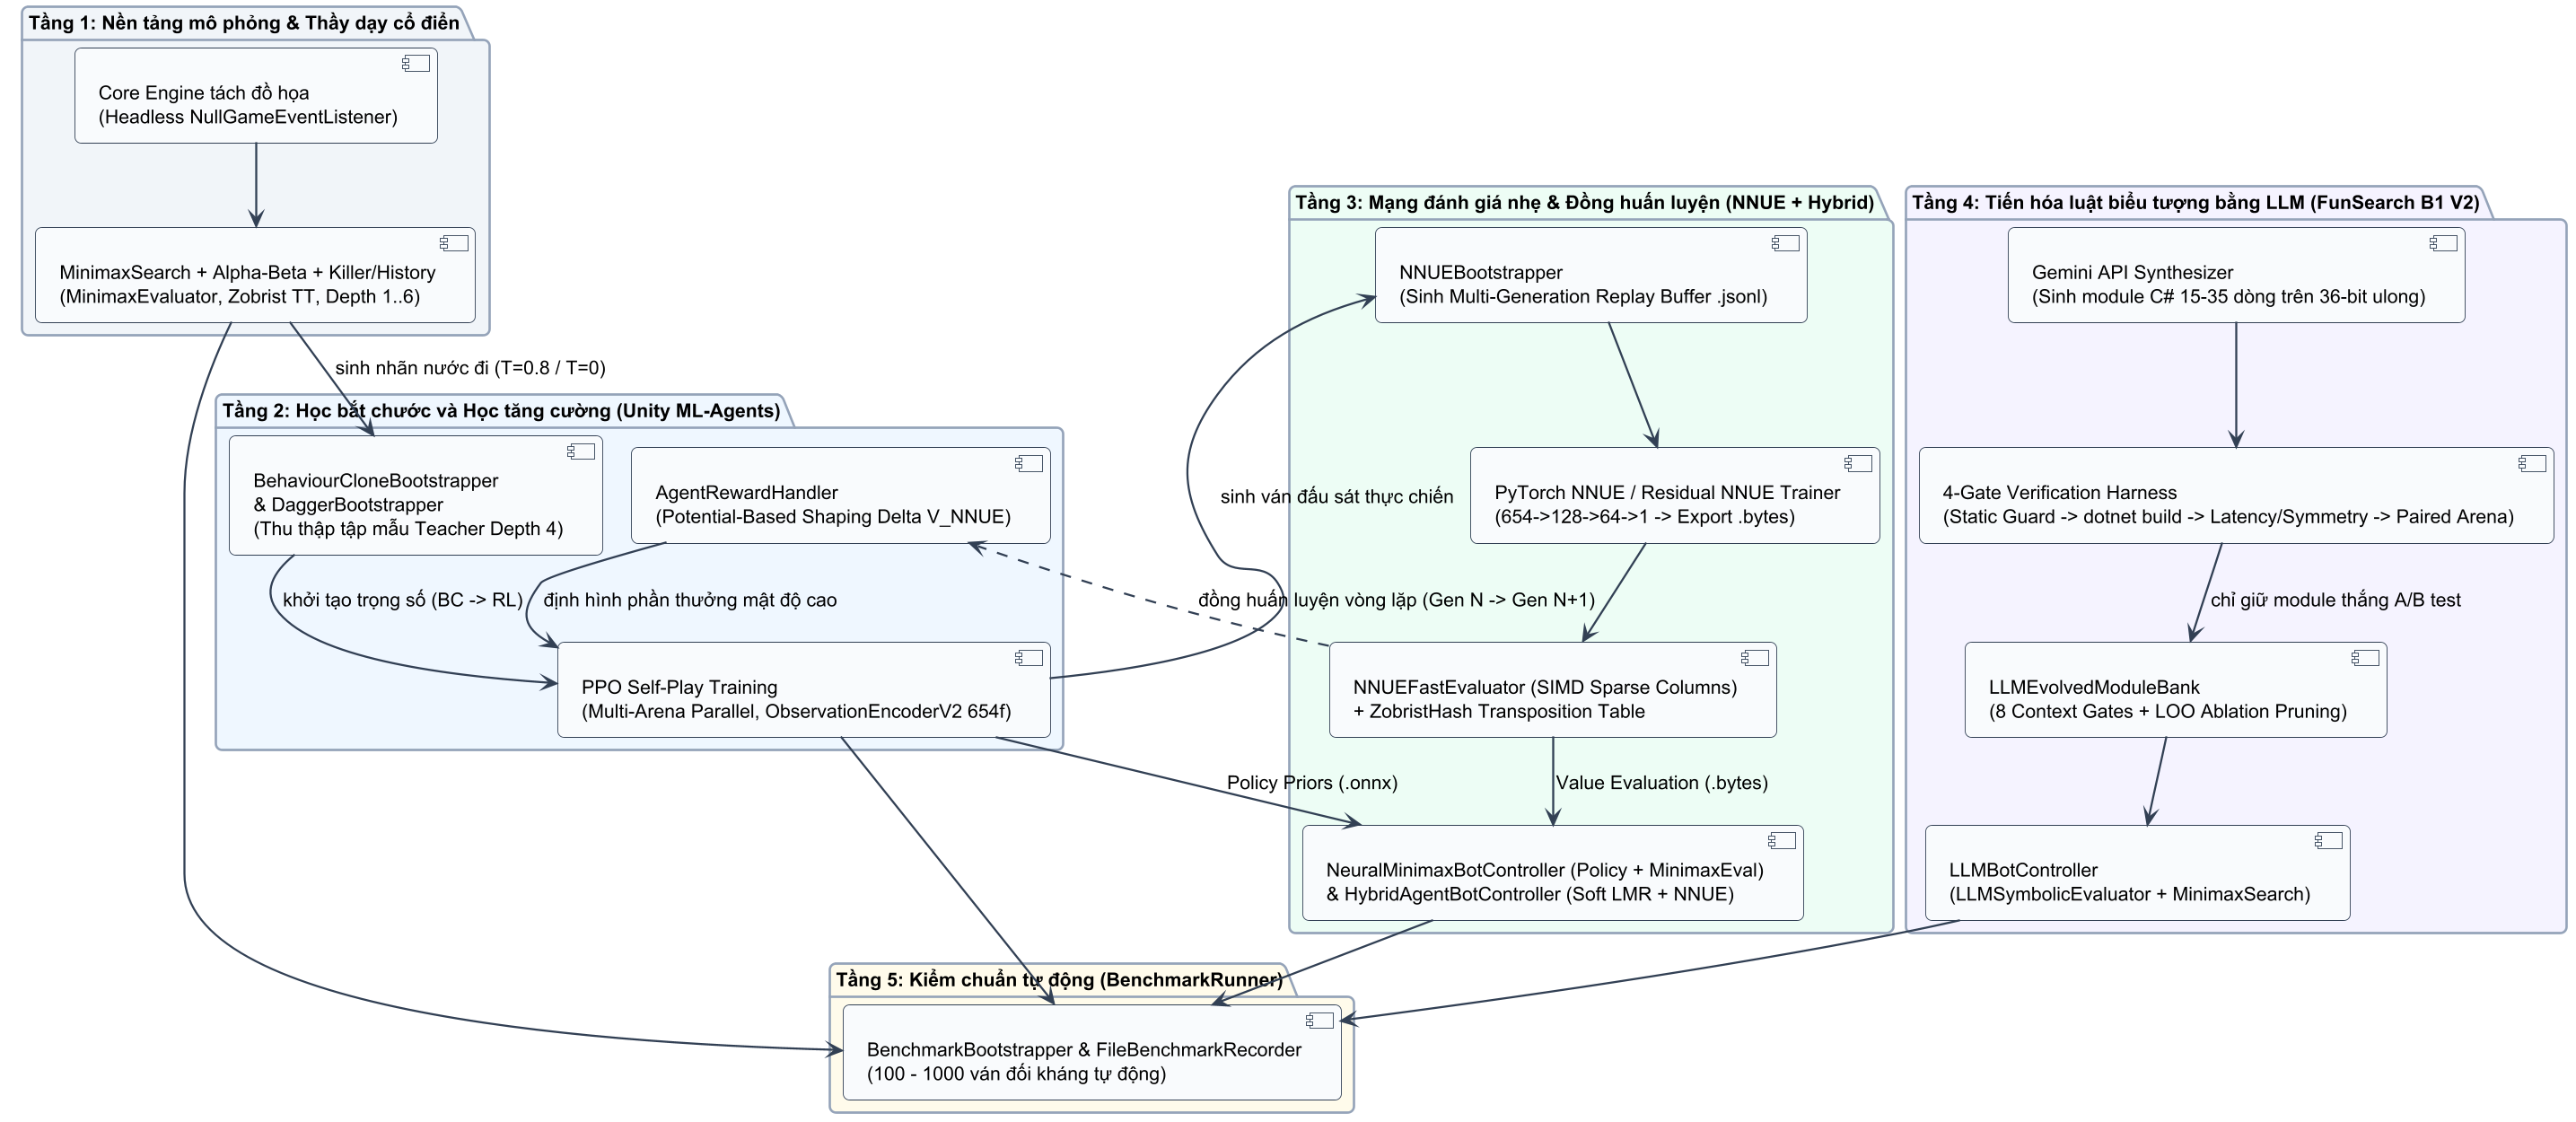
\includegraphics[width=0.96\textwidth]{Diagrams/images/09_pipeline_ai_training.png}
    \caption{Sơ đồ quy trình huấn luyện AI đa thế hệ (Minimax, BC/DAgger, PPO, NNUE, Hybrid và LLM)}
    \label{fig:pipeline_ai}
\end{figure}

Hình \ref{fig:pipeline_sc} trình bày kiến trúc tích hợp cục bộ giữa Unity 6 URP Client (\texttt{SCCharacterCreator}) và tiến trình Python \texttt{infer\_onnx.py} (chạy qua CLI subprocess và trao đổi tệp JSON/PNG) xử lý đồng thời hai nhánh Hình học khuôn mặt (Method B1 v2) và Chiếu Texture UV -- Khử bóng đối xứng (PyTorch3D Barycentric + Bilateral Symmetry Delighting + Multi-Band Pyramid + HRN).

\begin{figure}[H]
    \centering
    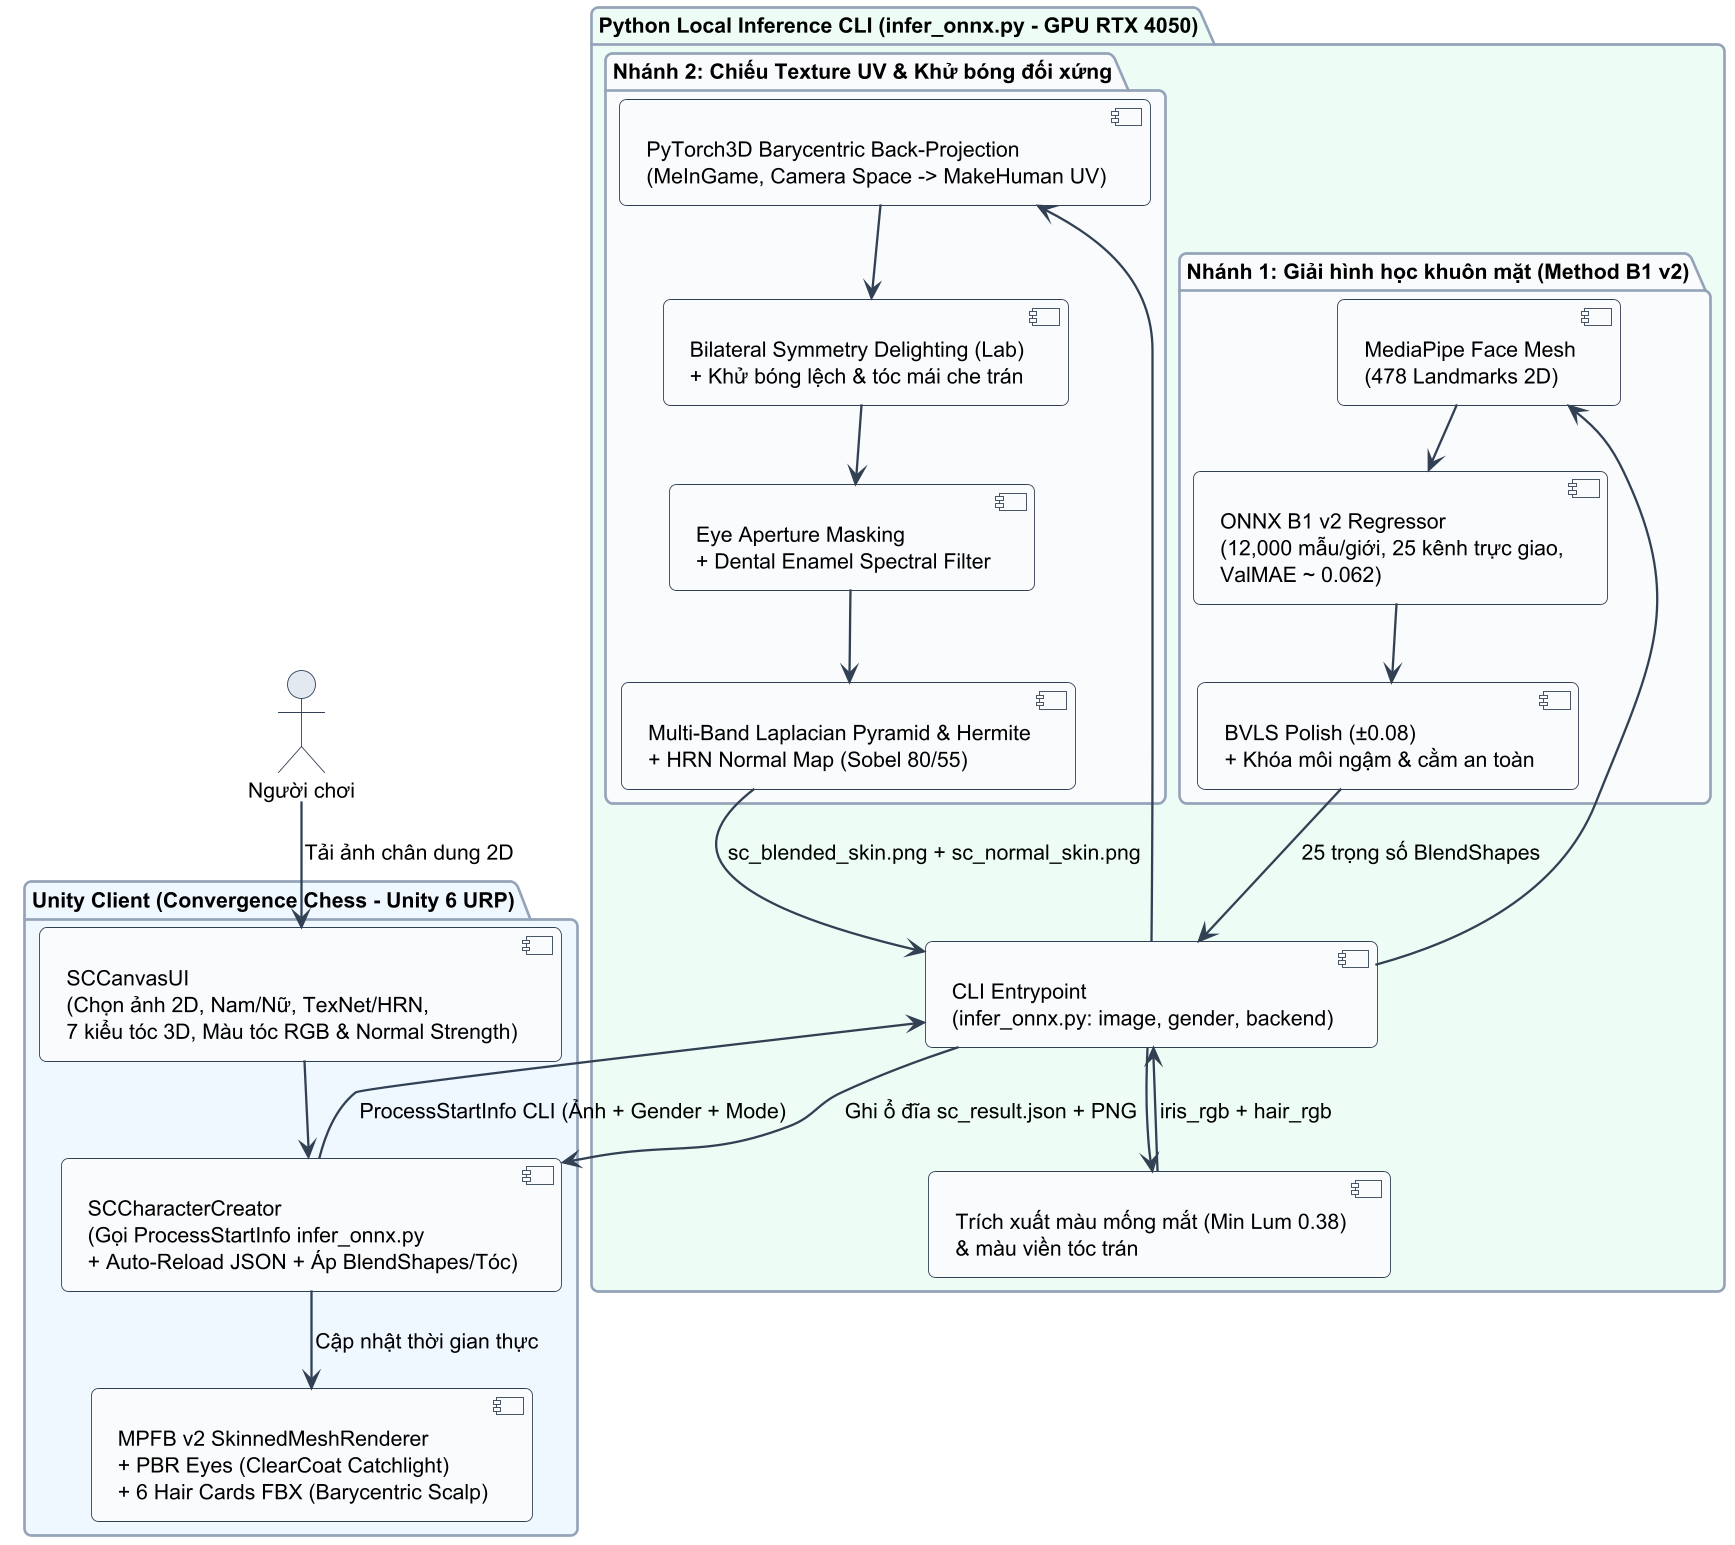
\includegraphics[width=0.88\textwidth]{Diagrams/images/10_pipeline_smart_customization.png}
    \caption{Sơ đồ kiến trúc xử lý cục bộ cho phân hệ tùy biến nhân vật 3D (Smart Customization)}
    \label{fig:pipeline_sc}
\end{figure}
